\documentclass[sigconf,anonymous]{acmart}
\usepackage{amsmath}
\usepackage{booktabs}
\usepackage{graphicx}
\usepackage{xcolor}
\usepackage{pifont}
\usepackage{multirow}
\usepackage{fancyvrb}
\usepackage{enumitem}
\setlist[itemize]{nosep,leftmargin=*}
\setlist[enumerate]{nosep,leftmargin=*}
\graphicspath{{./}{figures/}{../figures/}}
\setcopyright{none}
\settopmatter{printacmref=false}
\makeatletter
\@ifundefined{footnotetextcopyrightpermission}{}{%
  \renewcommand\footnotetextcopyrightpermission[1]{}%
}
\makeatother
\acmConference[Supplementary Material]{Supplementary Material}{2026}{Anonymous}
\acmYear{2026}
\copyrightyear{2026}
\acmISBN{}
\acmDOI{}

\begin{document}
\title{Supplementary Material for PlanGate}
\author{Anonymous}
\affiliation{\institution{Anonymous Institution}\country{}}
\email{anonymous@example.com}
\maketitle

\section{Artifact Evidence Packages Used in the Updated Paper}
\label{sec:artifact_evidence}

The updated paper text and the figures under \texttt{paper/figures} are generated from lightweight evidence packages under \texttt{artifact\_results/}. These packages intentionally contain only summary CSVs, validation metadata, hashes, and README files; they do not include full raw traces, provider keys, logs, virtual environments, or cache directories. Table~\ref{tab:artifact_evidence} records the evidence packages that feed the revised main-paper figures and mechanism discussion.

\begin{table}[h]
\centering
\caption{Lightweight evidence packages used by the updated paper text and \texttt{paper/figures}.}
\label{tab:artifact_evidence}
\small
\resizebox{\columnwidth}{!}{%
\begin{tabular}{@{}p{3.0cm}p{5.0cm}p{5.6cm}@{}}
\toprule
\textbf{Package} & \textbf{Primary CSVs} & \textbf{Validation signal} \\
\midrule
\texttt{mock\_regression\_p4\_refresh\_v1} & Exp1 core, Exp4 ablation, Exp8 discount, Exp10 adversarial & Refreshed mock regression summaries with no recorded row-level errors; used for core effective-goodput and cascade figures. \\
\texttt{throughput\_latency\_summary\_v1} & \texttt{throughput\_latency\_summary.csv}, \texttt{throughput\_latency\_agg.csv} & Covers Exp1/Exp5/Exp6/Exp10; \texttt{row\_count=200}, \texttt{agg\_row\_count=40}, required columns present. \\
\texttt{exp11\_newmechanismablation\_v1} & Exp11 summary and aggregate & Four variants, five repeats each; \texttt{row\_count=20}, \texttt{agg\_row\_count=4}, empty error column. \\
\texttt{p3\_failure\_mechanism\_ablation\_v1} & P3 failure/amendment summary and aggregate & Four variants, three repeats each; all client return codes and timeouts zero; signal checks confirm full recovery/amendment success and zeroed disabled mechanisms. \\
\texttt{p3\_failure\_amendment\_grid\_v1} & P3 grid summary and aggregate & Six $(failure,amendment)$ cells; majority of cells preserve the intended mechanism ordering, while low-failure boundary cells remain mixed rather than universally favorable to Full. \\
\texttt{selfhosted\_vllm\_stress\_c16w8\_tuned\_5gw\_v1} & \texttt{selfhosted\_vllm\_stress\_summary.csv}, \texttt{selfhosted\_vllm\_stress\_agg.csv} & Submitted self-hosted vLLM stress evidence with validation \texttt{errors=[]}; exactly the main-paper 5-gateway subset (ng/static/pp/rajomon/\texttt{plangate\_relaxed}), with \texttt{plangate\_real} omitted. \\
\texttt{selfhosted\_vllm\_profile\_sweep\_v1} & \texttt{selfhosted\_vllm\_profile\_sweep\_summary.csv}, \texttt{selfhosted\_vllm\_profile\_sweep\_agg.csv} & Multi-intensity self-hosted vLLM boundary evidence over $C{=}8/12/16/20$; explicitly retains the low-contention region where PlanGate is not always the top gateway. \\
\texttt{cloudlab\_random\_redis\_memory\_v1} & Redis-vs-memory CloudLab summary and aggregate & Random routing with Redis checkpoint/reservation state versus in-memory control; Redis records zero state misses while the control shows substantial state loss. \\
\texttt{statistical\_summary\_v1} & \texttt{statistical\_summary.csv}, \texttt{effect\_size\_summary.csv}, \texttt{claim\_summary.csv} & Bootstrap-based summary over existing artifact CSVs; validation now records \texttt{cloudlab\_included=true} with \texttt{errors=[]}. \\
\texttt{deepseek\_v4\_flash\_smoke\_v1} and \texttt{glm\_real\_llm\_c10\_refresh\_v1} & Provider smoke summaries & Real-provider compatibility and boundary evidence; used as support rather than primary dominance evidence. \\
\bottomrule
\end{tabular}}
\end{table}

The figure-generation script \texttt{scripts/build\_paper\_figures\_v2.py} reads only these artifact packages and writes deterministic PNG/PDF outputs into \texttt{paper/figures}. Re-running the script should overwrite figure files without creating new experimental data.

\section{Why Native API Gateways Are Insufficient}
\label{sec:envoy_analysis}

Production API gateways such as Envoy~\cite{envoy} and Kong~\cite{kong} provide mature request-oriented data planes: requests are routed, filtered, and rate-limited based primarily on per-client, per-route, or per-service policies. Their native rate-limiting abstractions are highly effective for transport-level overload control, but they do not directly express session-level admission decisions. Envoy's rate-limit service evaluates a descriptor tuple (domain, client ID, route) against a quota backend (e.g., Redis) without any notion of request sequence or session progress. Kong's rate-limiting plugin similarly enforces per-consumer quotas with no cross-request dependency tracking. Session affinity (sticky sessions) routes requests from the same client to the same backend, but it is a \emph{routing} mechanism, not an \emph{admission control} mechanism---it does not evaluate whether the backend can sustain a multi-step session to completion.

Table~\ref{tab:envoy_gap} decomposes the requirements for session commitment into five capabilities and maps them against what Envoy/Kong natively provide, what can be achieved via extensions, and which gaps require a custom stateful governance engine.

\begin{table}[h]
\caption{Session commitment requirements vs.\ native API gateway capabilities. \ding{55}\,=\,not natively supported; $\sim$\,=\,partially expressible with extensions; $\bigstar$\,=\,requires a custom stateful governance extension.}
\label{tab:envoy_gap}
\small
\resizebox{\columnwidth}{!}{%
\begin{tabular}{@{}p{2.6cm}ccp{3.2cm}@{}}
\toprule
\textbf{Requirement} & \textbf{Envoy/Kong} & \textbf{Extend?} & \textbf{Gap} \\
\midrule
\textbf{Session tracking} (cross-request state) & \ding{55} & $\sim$ & External store (e.g., Redis) can provide cross-request state, but introduces deployment-dependent lookup overhead and no native step counter \\
\textbf{Atomic admission} (DAG cost pre-flight) & \ding{55} & $\bigstar$ & Requires custom plan parser and admission state \\
\textbf{Temporal price isolation} (locked price snapshot) & \ding{55} & $\bigstar$ & Requires per-session locked price snapshots \\
\textbf{Continuation value} ($K^2$ sunk-cost discount) & \ding{55} & $\bigstar$ & Requires step-dependent admission pricing \\
\textbf{Governance intensity} (backend-load signal fusion) & \ding{55} & $\sim$ & Custom health-check can export load, but cannot feed into per-request pricing \\
\bottomrule
\end{tabular}}
\end{table}

\textbf{Empirical proxy.}
The SBAC baseline (session-based admission control via concurrent-session cap) and the Rajomon+SB baseline (Rajomon pricing with session bookkeeping) approximate the strongest plausible Envoy extensions: SBAC provides session tracking with binary admission (analogous to a per-session token bucket), and Rajomon+SB adds session awareness to dynamic pricing. Both achieve ABD $>56$\% versus PlanGate's 18.9\%, confirming that the missing capabilities---atomic admission, temporal isolation, and continuation value---are the decisive factors, not the transport layer.

\subsection{Envoy/Kong-Style Request-Level Proxy Baselines}
\label{sec:proxy_baselines}

To make the comparison with production API-gateway mechanisms more concrete, we also implement two request-level proxy approximations: \texttt{envoy\_approx} and \texttt{kong\_approx}. These are \emph{not} product benchmarks for Envoy or Kong. They are controlled approximations of common proxy primitives---global and route-level token buckets, in-flight caps, and per-consumer/session quotas---implemented inside the same experimental gateway stack so that they share the same backend, workload generator, and measurement path as the other baselines. By construction, they are request-local: they do not parse the declared DAG, reserve future steps, lock session prices, or provide session commitment.

\begin{table}[h]
\centering
\caption{Envoy/Kong-style proxy approximation baselines at $C{=}40$ (mean over 3 repeats). ABD\% is computed over admitted sessions. Request-level controls can limit traffic, but they do not provide session commitment.}
\label{tab:proxy_c40}
\small
\resizebox{\columnwidth}{!}{%
\begin{tabular}{@{}lrrrrrr@{}}
\toprule
\textbf{Gateway} & \textbf{Success} & \textbf{Rej0} & \textbf{Cascade} & \textbf{ABD\%} & \textbf{Success sess/s} & \textbf{Eff. GP/s} \\
\midrule
envoy\_approx  & 145.7 & 40.3  & 114.0 & 43.9 & 4.73 & 40.94 \\
kong\_approx   & 148.0 & 38.7  & 113.3 & 43.3 & 4.75 & 41.49 \\
NG             & 158.7 & 37.3  & 104.0 & 39.5 & 4.91 & 43.26 \\
SBAC           & 40.7  & 246.7 & 12.7  & 23.7 & 5.27 & 56.67 \\
SRL            & 42.7  & 236.3 & 21.0  & 32.9 & 5.75 & 48.95 \\
PlanGate       & 35.0  & 258.7 & 6.3   & 13.6 & 6.26 & 55.74 \\
\bottomrule
\end{tabular}}
\end{table}

Table~\ref{tab:proxy_c40} supports a constrained interpretation. The Envoy/Kong-style approximations retain high mid-session waste at moderate concurrency: at $C{=}40$, \texttt{envoy\_approx} and \texttt{kong\_approx} leave roughly 114 and 113 cascade-failed sessions per run, respectively, with admitted-session ABD above 43\%. PlanGate instead shifts most rejection to step~0 and reduces cascade failures to 6.3 sessions per run, but it does so through conservative admission rather than by creating additional backend capacity. Thus, the result should be read as evidence about governance granularity---request-level proxy control versus session-level commitment---not as a claim that PlanGate is a universal throughput winner.

A lightweight PlanGate sensitivity check at $C{=}40$ reinforces this tradeoff. With \texttt{price\_step=20}, increasing \texttt{max\_sessions} from 30 to 50 raises successful sessions from 34 to 62 and effective goodput from 37.61 to 63.38, while also increasing cascade failures from 4 to 8. With \texttt{price\_step=40}, the same max-session increase raises successful sessions from 38 to 66 and effective goodput from 42.21 to 62.27, with cascade failures increasing from 0 to 1. These four points show that more permissive admission can recover throughput, but only by allowing more mid-session risk; the proxy-baseline result is therefore best understood as an admission-vs-waste boundary characterization.

The self-hosted vLLM stress evidence is retained as a bounded diagnostic note rather than a universal proxy-baseline claim. In particular, the artifact retains a conservative PlanGate diagnostic profile for inspection, but the main-paper comparison uses a backend-capacity-tuned PlanGate display configuration for this specific saturated vLLM regime.

\section{Multi-Gateway Shared-State Validation Details}
\label{sec:multigateway_appendix}

This appendix section expands the main-paper multi-gateway result. The experiment is a controlled P\&S-only mock validation of shared reservation state. Each run submits $S{=}300$ declared-plan sessions to a 10-worker backend with PlanGate \texttt{max\_sessions=30}; we sweep $C\in\{20,40,60\}$ and repeat each configuration five times. The full run produces 60 per-step traces and 60 per-session traces under \texttt{results/exp\_multigateway\_shared\_state\_full/}. Quick validation runs are archived separately under \texttt{results/exp\_multigateway\_shared\_state\_quick/}.

Four deployment modes are used:
\begin{itemize}
  \item \textbf{Single-GW}: one gateway with process-local state.
  \item \textbf{2xGW-NoShare}: two gateways, independent process-local reservation state, random routing at each step.
  \item \textbf{2xGW-Sticky}: two gateways, independent process-local reservation state, but all steps from the same session are routed to the same gateway.
  \item \textbf{2xGW+Redis}: two gateways, random routing at each step, Redis-backed shared P\&S reservation state.
\end{itemize}

\begin{table}[h]
\centering
\caption{Full multi-gateway P\&S validation including the sticky-routing engineering baseline ($N{=}5$ repeats, $S{=}300$ sessions per run). StateMiss\% is the continuation semantic-failure rate. Sticky routing avoids misses by preserving routing locality, not by making state available across nodes.}
\label{tab:multigateway_full_appendix}
\small
\resizebox{\columnwidth}{!}{%
\begin{tabular}{@{}llrrrrrrr@{}}
\toprule
\textbf{Mode} & \textbf{C} & \textbf{Succ\%} & \textbf{Rej0\%} & \textbf{StateMiss\%} & \textbf{Cross\%} & \textbf{MaxAct} & \textbf{GP/s} & \textbf{P95(ms)} \\
\midrule
\multirow{3}{*}{Single-GW}
  & 20 & 17.6 & 82.4 & 0.0 & 0.0 & 17 & 5.96 & 2941 \\
  & 40 & 20.1 & 79.9 & 0.0 & 0.0 & 20 & 5.85 & 3301 \\
  & 60 & 18.6 & 81.4 & 0.0 & 0.0 & 20 & 5.79 & 3214 \\
\midrule
\multirow{3}{*}{2xGW-NoShare}
  & 20 & 3.1 & 68.5 & 28.5 & 28.5 & 3 & 1.06 & 2292 \\
  & 40 & 4.8 & 66.1 & 29.1 & 29.1 & 4 & 1.53 & 2701 \\
  & 60 & 3.9 & 66.1 & 30.1 & 30.1 & 3 & 1.25 & 1884 \\
\midrule
\multirow{3}{*}{2xGW-Sticky}
  & 20 & 44.4 & 55.6 & 0.0 & 0.0 & 20 & 6.76 & 4632 \\
  & 40 & 24.6 & 61.7 & 0.0 & 0.0 & 40 & 4.76 & 7851 \\
  & 60 & 21.9 & 72.2 & 0.0 & 0.0 & 43 & 5.36 & 6652 \\
\midrule
\multirow{3}{*}{2xGW+Redis}
  & 20 & 26.1 & 73.8 & 0.0 & 22.8 & 20 & 6.52 & 4606 \\
  & 40 & 22.1 & 77.3 & 0.0 & 19.7 & 31 & 6.51 & 5334 \\
  & 60 & 22.0 & 77.3 & 0.0 & 20.1 & 31 & 6.10 & 5934 \\
\bottomrule
\end{tabular}}
\end{table}

\textbf{Metric interpretation.} ABD is not the primary signal in this experiment because local random routing can fail by losing continuation state before it appears as an admitted-session cascade in the usual sense. We therefore report \emph{StateMiss\%}: the fraction of sessions whose later steps reach a gateway that lacks the required P\&S reservation state. The no-share random-routing control shows 28.5--30.1\% StateMiss, while Redis-backed shared state reduces StateMiss to 0.0\% even though 19.7--22.8\% of sessions execute on both gateway nodes. After the full run, Redis leak checks showed \texttt{pg:active\_sessions=0} and no residual \texttt{pg:admit:*} or \texttt{pg:res:*} keys.

\textbf{Scope.} This validation covers P\&S reservation state only. It does not evaluate shared ReAct progress, distributed reputation, dynamic price synchronization, node-failure recovery, or PlanGate-R recovery across gateway nodes.


% ================================================================
\section{Gateway Processing Overhead}
\label{sec:gateway_overhead_appendix}
% ================================================================

This appendix records the benchmark protocol used to support the main-paper overhead claim. The point is not that PlanGate is faster than a no-governance request path; the point is that the governance layer adds only microsecond-scale processing cost relative to tool execution and backend latency.

We report two complementary measurements. First, the Go in-process benchmark suite in \texttt{plangate/benchmark\_test.go} measures DAG validation, price computation, session lookup, the P\&S first-step admission path, and the standard \texttt{ServeHTTP} tool-call routes. Second, the live trace benchmark collects \texttt{X-Gateway-Latency-Us} from the gateway response header while exercising the same mock/light backend path used by the paper's controlled experiments. Because this header is gateway-observed service time and may include proxied backend/tool execution, we treat live traces as diagnostic only rather than primary evidence for pure gateway processing overhead. The live benchmark is organized by target gateway, concurrency, and cohort (successful admitted steps, step-0 rejections, all requests) for appendix diagnostics.

The benchmark outputs are written to \texttt{results/exp\_gateway\_overhead/}: the raw Go benchmark trace is saved as \texttt{go\_bench\_overhead.txt}, the parsed Go summary as \texttt{go\_bench\_overhead.csv}, the live aggregate as \texttt{gateway\_overhead\_agg.csv}, and the live percentile-sweep data as \texttt{gateway\_overhead\_cdf.csv}. The corresponding run command is provided in the artifact README, and the summary script is \texttt{scripts/\_compute\_gateway\_overhead\_stats.py}.

The interpretation is intentionally conservative: PlanGate's pure governance overhead claim is based on Go microbenchmarks, while live traces provide diagnostic context about gateway-observed service time. The throughput--latency gains reported in the main text therefore come from avoiding doomed sessions and queue pollution, not from a shorter per-request control path.


% ================================================================
\section{Supplementary Waste-Scaling Analysis}
\label{sec:theory_proof}
\label{app:theory}
% ================================================================

This appendix provides the complete formal treatment of the waste-scaling argument summarized in the main paper's continuation-discount rationale section. The theory is used to justify the shape of the ReAct continuation discount, not to claim an exact queueing model.

\subsection*{Cost Expectation Model}

To isolate the structural effect of governance granularity, we analyze a simplified model with uniform step cost ($c_i = c$), i.i.d.\ rejection probability ($q_k = q$), and geometrically distributed rejection timing. While real systems exhibit load-dependent $q$ and heterogeneous costs, this model captures the \emph{scaling behavior} of waste; the numerical validation below confirms the predicted orders of magnitude hold for practical $N \in [3,10]$.

Consider a session of $N$ uniform-cost steps, each consuming $c$ compute units. Under system load, each admission decision carries a rejection probability determined by the pricing strategy.

\textbf{Per-request pricing (no discount).}
Under stateless per-request pricing, each step independently faces rejection probability $q \in (0,1)$. A session passing step~0 is rejected at step~$k \geq 1$ with probability $(1{-}q)^{k-1}q$, wasting $k \cdot c$ invested compute. The \emph{expected waste per admitted session} is:
\begin{align}
E[W_{\text{req}}] &= c \cdot q \sum_{k=1}^{N-1} k\,(1{-}q)^{k-1} \notag\\
&= \frac{c\bigl[1 - N(1{-}q)^{N-1} + (N{-}1)(1{-}q)^N\bigr]}{q}
\label{eq:wreq}
\end{align}
For moderate rejection rates ($q \ll 1$), second-order Taylor expansion yields:
\begin{equation}
E[W_{\text{req}}] \approx c \cdot q \cdot \frac{N(N{-}1)}{2}
\label{eq:wreq_approx}
\end{equation}
i.e., expected waste grows \emph{quadratically} in session length~$N$.

\textbf{Session-level discounting.}
Under a discount function $d(k)$ with $d(0){=}1$ and $d(k) \leq 1$, the effective rejection probability at step~$k$ becomes $q_k = q \cdot d(k)$. For small~$q$, survival products $\prod_{i=1}^{k-1}(1{-}q_i) \approx 1$, giving:
\begin{equation}
E[W_d] \approx c \cdot q \sum_{k=1}^{N-1} k \cdot d(k)
\label{eq:wd}
\end{equation}

Table~\ref{tab:waste_scaling} summarizes waste scaling under four strategies.

\begin{table}[h]
\centering\small
\caption{Expected waste scaling under different discount strategies ($q \ll 1$). $H_m = \sum_{k=1}^{m} 1/k$ is the harmonic number.}
\label{tab:waste_scaling}
\resizebox{\columnwidth}{!}{%
\begin{tabular}{@{}llll@{}}
\toprule
\textbf{Strategy} & \textbf{$d(k)$} & \textbf{$\sum k\,d(k)$} & \textbf{$E[W]$ order} \\
\midrule
Per-request & $1$ & $N(N{-}1)/2$ & $O(N^2)$ \\
Linear & $\frac{1}{1+k\alpha}$ & $\leq (N{-}1)/\alpha$ & $O(N)$ \\
Quadratic ($K^2$) & $\frac{1}{1+k^2\alpha}$ & $\leq H_{N-1}/\alpha$ & $O(\ln N)$ \\
Budget reserv.\ (P\&S)$^*$ & $0\;(k{\geq}1)$ & $0$ & $O(1)$ \\
\bottomrule
\multicolumn{4}{@{}l}{\footnotesize $^*$Assumes reservation validity, backend availability, and plan accuracy;}\\
\multicolumn{4}{@{}l}{\footnotesize \phantom{$^*$}violations degrade gracefully to ReAct-mode $O(\ln N)$.}
\end{tabular}}
\end{table}

\textbf{Claim 1} (Waste reduction ratio).
\textit{Under the quadratic discount $d(k) = 1/(1{+}k^2\alpha)$ with $\alpha > 0$ and $q \ll 1$:}
\begin{align}
\frac{E[W_{\text{req}}]}{E[W_{K^2}]} &\geq \frac{\alpha\, N(N{-}1)}{2\,(\alpha + H_{N-1})} = \Theta\!\left(\frac{N^2}{\ln N}\right)
\label{eq:ratio}
\end{align}

\textit{Proof.}
For $q \ll 1$ the survival products satisfy $\prod_{i<k}(1{-}q_i)\approx 1$, so it suffices to compare the sums $S_{\text{req}}=\sum_{k=1}^{N-1}k$ and $S_{K^2}=\sum_{k=1}^{N-1}k/(1{+}k^2\alpha)$.

\emph{Upper bound on $S_{K^2}$.}
For $k\geq 1$, write $k/(1{+}k^2\alpha)\leq k/(k^2\alpha)=1/(k\alpha)$.
The first term contributes at most $1/(1{+}\alpha)\leq 1$.
Hence
$S_{K^2} \leq 1 + \frac{1}{\alpha}\sum_{k=2}^{N-1}\frac{1}{k}
       \leq 1 + \frac{H_{N-1}}{\alpha} = \frac{\alpha + H_{N-1}}{\alpha}$.

\emph{Integral confirmation.}
Because $f(x)=x/(1{+}x^2\alpha)$ is eventually decreasing,
\begin{align*}
\sum_{k=1}^{N-1}\frac{k}{1{+}k^2\alpha}
  &\leq \frac{1}{1{+}\alpha}+\int_{1}^{N-1}\!\frac{x}{1{+}x^2\alpha}\,dx \\
  &= \frac{1}{1{+}\alpha}+\frac{\ln\bigl(1{+}(N{-}1)^2\alpha\bigr)-\ln(1{+}\alpha)}{2\alpha} \\
  &= O\!\left(\frac{\ln N}{\alpha}\right).
\end{align*}
Dividing $S_{\text{req}}=N(N{-}1)/2$ by the upper bound on $S_{K^2}$ gives~(\ref{eq:ratio}).\hfill$\square$

\textbf{Numerical validation.}
For $N\in[3,10]$ with $\alpha{=}0.5$, evaluating the exact sums:
\begin{itemize}[nosep,leftmargin=*]
  \item Per-request: $S_{\text{req}}$ yields 3 ($N{=}3$) to 45 ($N{=}10$).
  \item Quadratic $K^2$: $S_{K^2}=\sum k/(1{+}0.5k^2)$ yields 1.33 ($N{=}3$) to 3.75 ($N{=}10$).
  \item \textbf{Reduction ratio}: $2.3\times$ at $N{=}3$; $4.3\times$ at $N{=}5$; $7.0\times$ at $N{=}7$; $12.0\times$ at $N{=}10$.
\end{itemize}
The ratio grows with session length---explaining the amplified long-tail benefits---and is already practically significant ($\geq 2\times$) at the shortest sessions in our workload.

\textbf{Qualitative design arguments.}
In PlanGate's P\&S mode, sessions declare a DAG at admission; budget reservation prevents price-induced rejection within the declared plan scope under the stated assumptions. ReAct sessions cannot declare future steps, so risk exposure $R(K) = \sum_{i=1}^{K} c_i$ grows with each step and the discount function directly controls the tradeoff. The convex $d(K)=1/(1+K^2\alpha)$ captures the acceleration: at $K{=}3$ with $\alpha{=}0.5$, the effective price drops to 18\% of base. A linear discount $d(K)=1/(1+K\alpha)$ achieves only $O(N)$ waste; a constant discount ignores sunk cost entirely. The refreshed discount-function ablation in the main paper should therefore be read as diagnostic sensitivity evidence rather than as proof that $K^2$ is the empirical winner in every workload: in the current artifact, exponential and linear variants complete slightly more sessions and achieve higher effective goodput than quadratic and logarithmic, while cascade counts remain clustered and JFI is effectively 1.0 for all four variants. We retain the quadratic form as the default because it is the simplest convex schedule with predictable monotone growth and conservative continuation pricing, not because Exp8 currently shows it dominating all alternatives.


% ================================================================
\section{Sensitivity to Load-Modulated Continuation Discount}
\label{sec:beta-sensitivity}
\label{app:beta}
% ================================================================

PlanGate uses a load-modulated sunk-cost coefficient for ReAct continuation pricing:
\begin{equation}
\alpha_{\mathrm{eff}}=\alpha\bigl(1+\beta(1-I(t))\bigr),
\end{equation}
where $I(t)\in[0,1]$ is the governance intensity and $\beta$ controls how much additional slack is granted under lighter load. The default $\beta{=}1$ recovers the original $\alpha(2-I(t))$ form and bounds $\alpha_{\mathrm{eff}}\in[\alpha,2\alpha]$.

Table~\ref{tab:beta-ablation} reports a pure-ReAct mock ablation over $\beta\in\{0,0.5,1,2,3\}$ with the quadratic $K^2$ discount. All settings complete the same number of sessions, indicating that the load-modulation constant does not determine overall throughput. Larger $\beta$ values slightly reduce cascades and ABD, but also increase step-0 rejections and can reduce effective goodput or fairness. We therefore use $\beta{=}1$ as a conservative default rather than claiming it is globally optimal.

\begin{table}[h]
\centering
\caption{Sensitivity to the load-modulation coefficient $\beta$ in
$\alpha_{\mathrm{eff}}=\alpha(1+\beta(1-I(t)))$ under a pure-ReAct mock workload (500 sessions, 200 concurrency, 5 repeats). The default $\beta{=}1$ recovers the original $\alpha(2-I(t))$ form.}
\label{tab:beta-ablation}
\small
\resizebox{\columnwidth}{!}{%
\begin{tabular}{@{}crrrrrrr@{}}
\toprule
$\beta$ & Succ. & Rej\textsubscript{0} & Cascade & ABD\textsubscript{ReAct}\% & GP/s & P95\,ms & JFI \\
\midrule
0.0 & 30.0 & 456.8 & $13.2\pm2.2$ & 30.4 & 24.67 & 800 & 0.793 \\
0.5 & 30.0 & 457.8 & $12.2\pm4.0$ & 28.4 & 23.65 & 807 & 0.768 \\
1.0 & 30.0 & 456.0 & $14.0\pm3.7$ & 31.4 & 23.76 & 832 & 0.763 \\
2.0 & 30.0 & 459.2 & $10.8\pm4.5$ & 25.8 & 23.41 & 758 & 0.774 \\
3.0 & 30.0 & 459.2 & $10.8\pm3.0$ & 26.1 & 22.95 & 821 & 0.743 \\
\bottomrule
\end{tabular}}
\end{table}

The sweep shows that the continuation-pricing mechanism is not brittle to the specific constant. Setting $\beta{=}0$ removes load-dependent slack amplification while preserving the $K^2$ progress discount; setting $\beta{>}1$ makes the policy more generous to continuing sessions under lower load. The completion count is identical across all settings, so most of the benefit comes from the quadratic progress discount rather than from a finely tuned modulation constant. Larger $\beta$ values reduce cascades slightly but provide only marginal gains while increasing rejection aggressiveness or reducing fairness. We therefore keep $\beta{=}1$ as a simple and conservative operating point.


% ================================================================
\section{Practical Abuse Control: Full Implementation}
\label{sec:reputation_appendix}
\label{app:reputation}
% ================================================================

PlanGate's admission control relies on client-declared headers (\texttt{X-Total-Budget}, \texttt{X-Plan-DAG}), creating a zero-trust vulnerability: adversarial agents may inflate budgets or submit fraudulent DAGs to monopolize session slots. To mitigate this, PlanGate incorporates a lightweight reputation system.

\textbf{Trust Score and Enforcement.}
Each agent $a$ (identified by \texttt{X-Agent-ID}) has a trust score $T_a \in [0, 1]$, updated via EWMA after each session:

\begin{equation}
T_a^{(t+1)} = \rho \cdot T_a^{(t)} + (1 - \rho) \cdot r^{(t)}
\end{equation}

\noindent where $\rho = 0.98$ (learning rate $\eta{=}0.02$), $r^{(t)} \in \{0, 1\}$ is the session outcome (1 = success, 0 = failure), and new agents start at $T_a = 1.0$ (optimistic initialization).Budget or DAG violations additionally incur a flat penalty $T_a \mathrel{-}= \delta{=}0.15$. Two enforcement levels: (1)~any agent with $T_a < 1$ has its declared budget scaled ($B \leftarrow B \times T_a$), equivalent to tighter admission; (2)~agents with $T_a < \tau_{\text{ban}}{=}0.3$ are banned (HTTP~403). The flat penalty ensures 5 consecutive violations from a fully-trusted start trigger a ban ($T = 1.0 - 5{\times}0.15 = 0.25 < 0.3$). This mechanism is not a full Sybil-resistant identity system, but prevents naive slot monopolization while keeping admission decisions inexpensive.

\textbf{Adversarial Robustness Experiment.}
To validate the reputation mechanism, we inject 10\% adversarial agents (${10\times}$ inflated budgets, 15--20-step DAGs) into a 500-session workload at 200 concurrency, averaged over 5 runs. (The artifact script for this experiment is \texttt{exp10}.)

\begin{table}[h]
\caption{Adversarial robustness (500 sessions, 10\% adversarial agents, $N{=}5$).}
\label{tab:adversarial}
\small
\begin{tabular}{@{}lrrrr@{}}
\toprule
\textbf{Gateway} & \textbf{Succ.} & \textbf{Casc.} & \textbf{Eff.GP/s} & \textbf{JFI$_s$} \\
\midrule
NG        & 28.8  & 119.4  & 18.8  & 0.762 \\
SRL       & 38.0  & 113.2  & 27.3  & 0.706 \\
SBAC      & 52.0  & 39.4   & 41.8  & 0.748 \\
\textbf{PlanGate} & \textbf{72.6} & \textbf{1.0} & \textbf{58.0} & 0.656 \\
\bottomrule
\end{tabular}
\end{table}

PlanGate achieves 72.6 successful tasks ($2.5\times$ NG's 28.8) with only 1.0 cascade failure. The EWMA-based trust score drops below the ban threshold ($\tau{=}0.3$) after initial oversized DAGs trigger cascades, causing subsequent adversarial requests to be rejected at Step~0. PlanGate's lower JFI$_s$ (0.656 vs.\ NG's 0.762) reflects deliberate discrimination against adversarial agents---a desirable fairness--security tradeoff.

\begin{figure}[h]
\centering
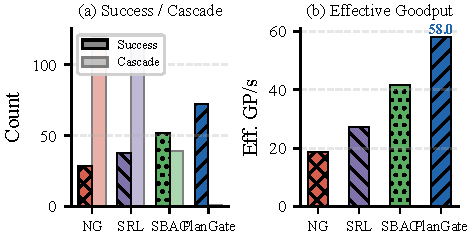
\includegraphics[width=\columnwidth]{exp10_adversarial}
\caption{Adversarial robustness (10\% malicious agents). PlanGate achieves $2.5\times$ more successful tasks than NG with only 1.0 cascade failure.}
\label{fig:exp10_adversarial}
\end{figure}

\vspace{1em}

% ================================================================
\section{Self-Hosted vLLM: High-Contention Regime ($C{=}16$)}
\label{sec:selfhosted_c16}
\label{app:vllm-high}
% ================================================================

The self-hosted vLLM high-contention experiment is reported in the main paper's self-hosted vLLM section, self-hosted vLLM table, and self-hosted vLLM figure. The protocol is: $N{=}3$ repeats, 80 agents, $C{=}16$, burst arrival (12 per burst with 5\,s gap), \texttt{max\_steps=8}, 8 backend/GPU workers, and vLLM \texttt{max-num-seqs=8}. The submitted artifact contains the main-paper 5-gateway display subset: \texttt{ng}, \texttt{static}, \texttt{pp}, \texttt{rajomon}, and \texttt{plangate\_relaxed} (shown as PlanGate (tuned)); it does not include \texttt{plangate\_real}. A conservative diagnostic profile was used during local sensitivity checking but is not included in the submitted vLLM artifact.

% ================================================================
\section{Self-Hosted vLLM Multi-Intensity Sweep}
\label{sec:selfhosted_profile_appendix}
% ================================================================

Table~\ref{tab:selfhosted_profile_appendix} reproduces the complete aggregate CSV from \texttt{artifact\_results/selfhosted\_vllm\_profile\_sweep\_v1}. The main-paper interpretation is intentionally bounded: the $C{=}8$ row set preserves the low-contention region where PlanGate (tuned) is not the top success-rate gateway, while the $C{=}16/20$ rows show the harsher saturation regime where its success/ABD trade-off improves relative to several baselines.

\begin{figure}[h]
\centering
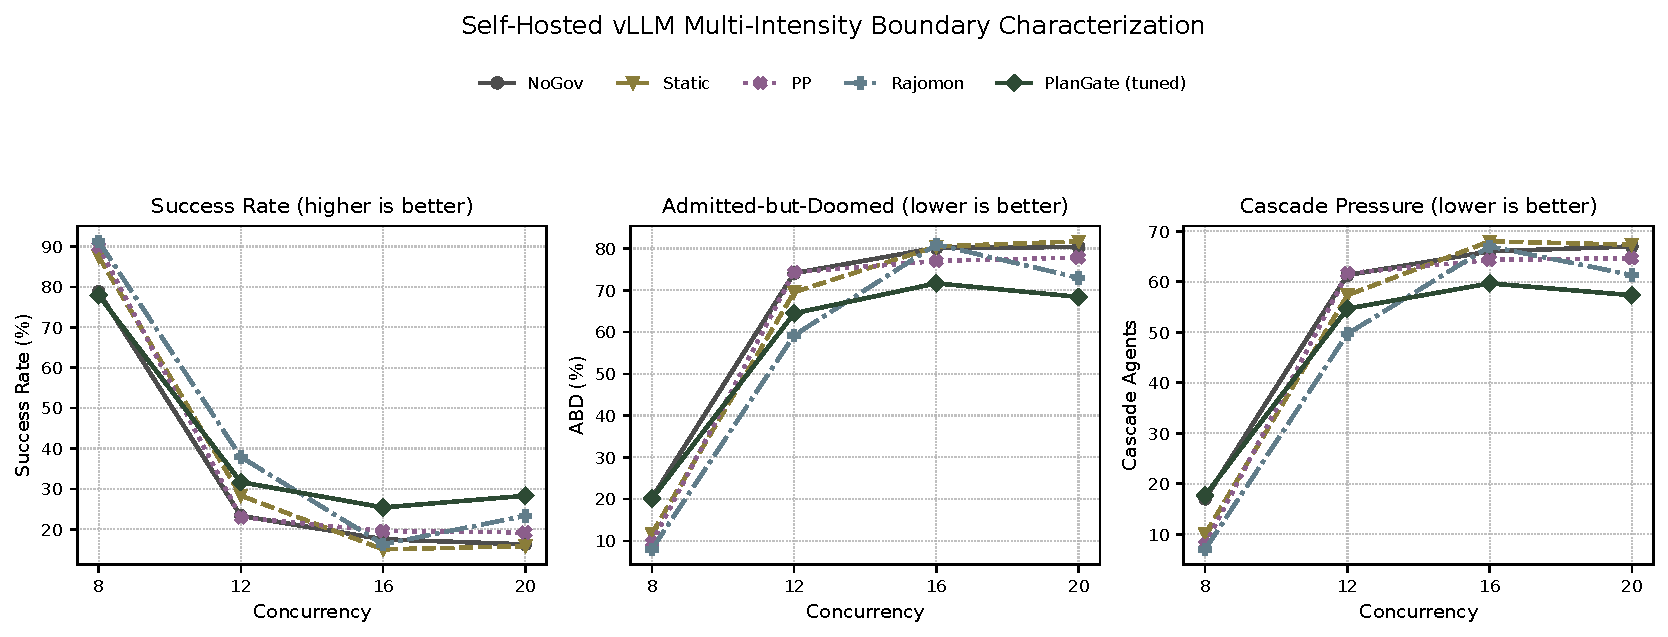
\includegraphics[width=\columnwidth]{fig_selfhosted_vllm_profile_sweep}
\caption{Full self-hosted vLLM profile sweep figure generated from \texttt{selfhosted\_vllm\_profile\_sweep\_agg.csv}.}
\label{fig:selfhosted_profile_appendix}
\end{figure}

\begin{table*}[h]
\centering
\caption{Complete self-hosted vLLM profile-sweep aggregate table from \texttt{artifact\_results/selfhosted\_vllm\_profile\_sweep\_v1/selfhosted\_vllm\_profile\_sweep\_agg.csv}. P95 is reported in seconds.}
\label{tab:selfhosted_profile_appendix}
\small
\resizebox{\textwidth}{!}{%
\begin{tabular}{@{}rrrcccc@{}}
\toprule
\textbf{C} & \textbf{Gateway} & \textbf{Runs} & \textbf{Succ.\%} & \textbf{ABD\%} & \textbf{Cascade} & \textbf{P95 (s)} \\
\midrule
8 & ng & 3 & 78.77 & 20.23 & 17.00 & 199.7 \\
8 & plangate\_relaxed & 3 & 77.93 & 20.10 & 17.67 & 206.3 \\
8 & pp & 3 & 90.00 & 9.63 & 8.00 & 205.8 \\
8 & rajomon & 3 & 91.27 & 7.97 & 7.00 & 204.9 \\
8 & static & 3 & 87.50 & 11.73 & 10.00 & 225.4 \\
12 & ng & 3 & 23.33 & 74.10 & 61.33 & 178.5 \\
12 & plangate\_relaxed & 3 & 31.67 & 64.50 & 54.67 & 176.2 \\
12 & pp & 3 & 22.93 & 74.33 & 61.67 & 176.6 \\
12 & rajomon & 3 & 37.90 & 59.23 & 49.67 & 205.3 \\
12 & static & 3 & 28.33 & 69.57 & 57.33 & 176.4 \\
16 & ng & 3 & 17.53 & 80.17 & 66.00 & 187.6 \\
16 & plangate\_relaxed & 3 & 25.40 & 71.67 & 59.67 & 185.7 \\
16 & pp & 3 & 19.57 & 77.03 & 64.33 & 226.4 \\
16 & rajomon & 3 & 16.27 & 80.97 & 67.00 & 188.1 \\
16 & static & 3 & 15.03 & 80.50 & 68.00 & 175.8 \\
20 & ng & 3 & 16.27 & 80.37 & 67.00 & 186.8 \\
20 & plangate\_relaxed & 3 & 28.30 & 68.43 & 57.33 & 163.7 \\
20 & pp & 3 & 19.20 & 77.87 & 64.67 & 157.8 \\
20 & rajomon & 3 & 23.33 & 73.00 & 61.33 & 194.2 \\
20 & static & 3 & 15.83 & 81.73 & 67.33 & 173.9 \\
\bottomrule
\end{tabular}}
\end{table*}

% ================================================================
\section{P3 Failure/Amendment Grid Aggregate}
\label{sec:p3_grid_appendix}
% ================================================================

Table~\ref{tab:p3_grid_appendix} reproduces the complete aggregate CSV from \texttt{artifact\_results/p3\_failure\_amendment\_grid\_v1}. Figure~\ref{fig:p3_grid_appendix} visualizes the same boundary: the dominant qualitative signal is stable mechanism activation, not that Full wins every cell on every aggregate metric.

\begin{figure}[h]
\centering
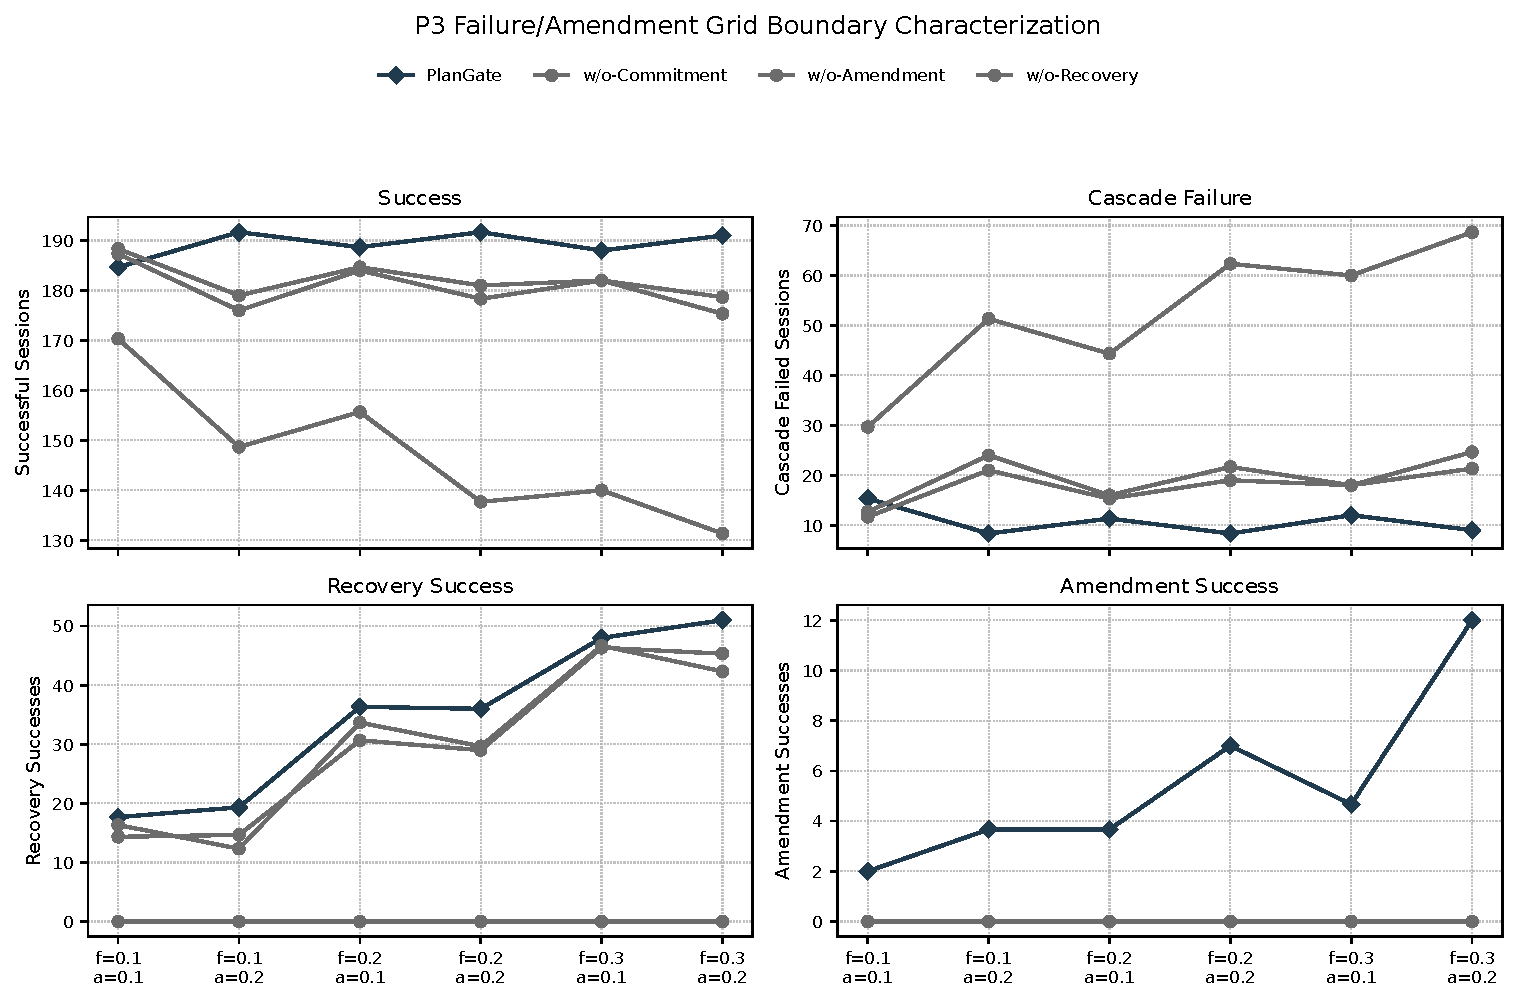
\includegraphics[width=\columnwidth]{fig_p3_failure_amendment_grid}
\caption{P3 failure/amendment grid figure generated from \texttt{p3\_failure\_amendment\_grid\_agg.csv}.}
\label{fig:p3_grid_appendix}
\end{figure}

\begin{table*}[h]
\centering
\caption{Complete P3 failure/amendment grid aggregate from \texttt{artifact\_results/p3\_failure\_amendment\_grid\_v1/p3\_failure\_amendment\_grid\_agg.csv}.}
\label{tab:p3_grid_appendix}
\small
\resizebox{\textwidth}{!}{%
\begin{tabular}{@{}cccrrrrr@{}}
\toprule
\textbf{Fail.} & \textbf{Amend.} & \textbf{Gateway} & \textbf{Runs} & \textbf{Success} & \textbf{Cascade} & \textbf{Recovery} & \textbf{Amendment} \\
\midrule
0.1 & 0.1 & plangate\_full & 3 & 184.7 & 15.3 & 17.7 & 2.0 \\
0.1 & 0.1 & wo\_amendment & 3 & 188.3 & 11.7 & 16.3 & 0.0 \\
0.1 & 0.1 & wo\_commitment & 3 & 187.3 & 12.7 & 14.3 & 0.0 \\
0.1 & 0.1 & wo\_recovery & 3 & 170.3 & 29.7 & 0.0 & 0.0 \\
0.1 & 0.2 & plangate\_full & 3 & 191.7 & 8.3 & 19.3 & 3.7 \\
0.1 & 0.2 & wo\_amendment & 3 & 179.0 & 21.0 & 12.3 & 0.0 \\
0.1 & 0.2 & wo\_commitment & 3 & 176.0 & 24.0 & 14.7 & 0.0 \\
0.1 & 0.2 & wo\_recovery & 3 & 148.7 & 51.3 & 0.0 & 0.0 \\
0.2 & 0.1 & plangate\_full & 3 & 188.7 & 11.3 & 36.3 & 3.7 \\
0.2 & 0.1 & wo\_amendment & 3 & 184.7 & 15.3 & 33.7 & 0.0 \\
0.2 & 0.1 & wo\_commitment & 3 & 184.0 & 16.0 & 30.7 & 0.0 \\
0.2 & 0.1 & wo\_recovery & 3 & 155.7 & 44.3 & 0.0 & 0.0 \\
0.2 & 0.2 & plangate\_full & 3 & 191.7 & 8.3 & 36.0 & 7.0 \\
0.2 & 0.2 & wo\_amendment & 3 & 181.0 & 19.0 & 29.7 & 0.0 \\
0.2 & 0.2 & wo\_commitment & 3 & 178.3 & 21.7 & 29.0 & 0.0 \\
0.2 & 0.2 & wo\_recovery & 3 & 137.7 & 62.3 & 0.0 & 0.0 \\
0.3 & 0.1 & plangate\_full & 3 & 188.0 & 12.0 & 48.0 & 4.7 \\
0.3 & 0.1 & wo\_amendment & 3 & 182.0 & 18.0 & 46.7 & 0.0 \\
0.3 & 0.1 & wo\_commitment & 3 & 182.0 & 18.0 & 46.3 & 0.0 \\
0.3 & 0.1 & wo\_recovery & 3 & 140.0 & 60.0 & 0.0 & 0.0 \\
0.3 & 0.2 & plangate\_full & 3 & 191.0 & 9.0 & 51.0 & 12.0 \\
0.3 & 0.2 & wo\_amendment & 3 & 175.3 & 24.7 & 42.3 & 0.0 \\
0.3 & 0.2 & wo\_commitment & 3 & 178.7 & 21.3 & 45.3 & 0.0 \\
0.3 & 0.2 & wo\_recovery & 3 & 131.3 & 68.7 & 0.0 & 0.0 \\
\bottomrule
\end{tabular}}
\end{table*}

% ================================================================
\section{CloudLab Random-Routing Redis vs Memory}
\label{sec:cloudlab_random_redis_memory_appendix}
% ================================================================

Table~\ref{tab:cloudlab_random_redis_memory_appendix} reproduces the per-run summary CSV from \texttt{artifact\_results/cloudlab\_random\_redis\_memory\_v1}. The Redis arm is the correctness arm and the in-memory arm is the diagnostic control. The table should be read narrowly as shared-state lookup evidence under random routing.

\begin{table*}[h]
\centering
\caption{Complete CloudLab Redis-vs-memory per-run summary from \texttt{artifact\_results/cloudlab\_random\_redis\_memory\_v1/cloudlab\_random\_redis\_memory\_summary.csv}.}
\label{tab:cloudlab_random_redis_memory_appendix}
\small
\resizebox{\textwidth}{!}{%
\begin{tabular}{@{}lrrrrrrr@{}}
\toprule
\textbf{Store} & \textbf{Repeat} & \textbf{Cross-node} & \textbf{StateMiss} & \textbf{DupAdm} & \textbf{Invalid} & \textbf{Mismatch} & \textbf{Expired} \\
\midrule
memory & 1 & 4049 & 3215 & 0 & 0 & 0 & 0 \\
memory & 2 & 4190 & 3330 & 0 & 0 & 0 & 0 \\
memory & 3 & 4159 & 3268 & 0 & 0 & 0 & 0 \\
redis & 1 & 7381 & 0 & 0 & 0 & 0 & 0 \\
redis & 2 & 7057 & 0 & 0 & 0 & 0 & 0 \\
redis & 3 & 7439 & 0 & 0 & 0 & 0 & 0 \\
\bottomrule
\end{tabular}}
\end{table*}

% ================================================================
\section{Full Statistical Summary Listings}
\label{sec:statistical_summary_appendix}
% ================================================================

The complete statistical-summary and effect-size tables are preserved as machine-readable appendix listings under \texttt{artifact\_results/statistical\_summary\_v1}. They are reproduced directly below to avoid manual transcription drift. These listings should be read with the same evidence hierarchy as the main text: CloudLab rows are state-consistency evidence, provider rows remain boundary evidence if added later, and diagnostics such as Exp8 remain explicitly labeled diagnostic.

\subsection*{Full \texttt{statistical\_summary.csv}}
\IfFileExists{../../artifact_results/statistical_summary_v1/statistical_summary.csv}{%
{\scriptsize\VerbatimInput{../../artifact_results/statistical_summary_v1/statistical_summary.csv}}%
}{\textbf{Missing file:} \texttt{../../artifact\_results/statistical\_summary\_v1/statistical\_summary.csv}}

\subsection*{Full \texttt{effect\_size\_summary.csv}}
\IfFileExists{../../artifact_results/statistical_summary_v1/effect_size_summary.csv}{%
{\scriptsize\VerbatimInput{../../artifact_results/statistical_summary_v1/effect_size_summary.csv}}%
}{\textbf{Missing file:} \texttt{../../artifact\_results/statistical\_summary\_v1/effect\_size\_summary.csv}}


% ================================================================
\section{Implementation Details}
\label{sec:impl_details}
% ================================================================

Table~\ref{tab:impl} summarizes the implementation scope. PlanGate is implemented in approximately 3,500 lines of Go (gateway and governor) and 2,000 lines of Python (backend, agents, and evaluation scripts).

\begin{table}[h]
\caption{Implementation components and lines of code.}
\label{tab:impl}
\small
\begin{tabular}{@{}llr@{}}
\toprule
\textbf{Component} & \textbf{Language} & \textbf{LoC} \\
\midrule
PlanGate Gateway & Go & $\sim$2,000 \\
MCPGovernor Engine & Go & $\sim$800 \\
Baseline Gateways (3) & Go & $\sim$500 \\
MCP Backend Server & Python & $\sim$600 \\
Agent Clients & Python & $\sim$800 \\
Evaluation Scripts & Python & $\sim$600 \\
\bottomrule
\end{tabular}
\end{table}

\textbf{Evaluation Infrastructure.} The test harness manages experiment lifecycle: building the Go gateway, launching the Python backend, generating load via concurrent agent clients, and collecting per-session and per-step metrics. CPU isolation is enforced via \texttt{taskset}: cores 0--3 for load generation, 4--7 for the gateway, and 8--15 for the backend. The anonymized artifact contains gateway source, Python backend, agent clients, experiment scripts, and reproduction instructions for no-key controlled mock experiments on a single machine. Provider-backed real-LLM experiments require API credentials and provider availability for live reruns. Optional supplementary materials for artifact evaluation are documented separately in the artifact README.

% ================================================================
\section{PlanGate-R: Recovery Sensitivity to Failure Rate}
\label{sec:recovery-appendix}
% ================================================================

Table~\ref{tab:plangate_r_sensitivity} extends the controlled runtime recovery evaluation of the main paper (Section~5.12) across three injected failure rates.
All settings: $S{=}50$, $N{=}5$, failure injected at step~2, 5 independent seeds per rate, P\&S mock, no real LLM.
These are controlled mock runtime results only; they do not represent real-LLM or production recovery performance, and are not ReAct semantic recovery experiments.

The table confirms that the replay-waste advantage of PlanGate-R over naive retry scales with the injected failure rate.
At $r{=}0.1$, when failures occur rarely, PlanGate-base already achieves $0.912$ success and avoided replay is modest ($8.8$~calls/run).
At $r{=}0.5$, PlanGate-base success drops to $0.476$ and avoided replay reaches $52.4$~calls/run.
In this controlled fail-once mock runtime, PlanGate-R maintains $1.000\pm0.000$ eventual success across the tested rates.

\begin{table}[h]
\centering
\caption{PlanGate-R sensitivity to injected failure rate (controlled mock runtime, P\&S only,
  $S{=}50$, $N{=}5$, failure injected at step~2, 5 seeds per rate;
  mock handlers, no real LLM, no ReAct semantic recovery).
  \emph{Waste Steps} = tool-call steps that do not contribute to the final successful trajectory.
  \emph{Avoided Replay} = calls saved by PlanGate-R vs.\ naive retry (mean over seeds).}
\label{tab:plangate_r_sensitivity}
\small
\resizebox{\columnwidth}{!}{%
\begin{tabular}{@{}clrrrr@{}}
\toprule
\textbf{Rate} & \textbf{Policy}           & \textbf{Success Rate}    & \textbf{Tool Calls}        & \textbf{Waste Steps}       & \textbf{Avoided Replay} \\
\midrule
\multirow{3}{*}{0.1}
  & PlanGate-base       & $0.912\pm0.033$          & $241.2\pm3.3$              & $13.2\pm5.0$               & $0.0$ \\
  & Naive retry         & $1.000\pm0.000$          & $263.2\pm5.0$              & $13.2\pm5.0$               & $0.0$ \\
  & \textbf{PlanGate-R} & $1.000\pm0.000$          & $\mathbf{254.4\pm1.7}$     & $\mathbf{4.4\pm1.7}$       & $\mathbf{8.8}$ \\
\midrule
\multirow{3}{*}{0.3}
  & PlanGate-base       & $0.704\pm0.055$          & $220.4\pm5.5$              & $44.4\pm8.3$               & $0.0$ \\
  & Naive retry         & $1.000\pm0.000$          & $294.4\pm8.3$              & $44.4\pm8.3$               & $0.0$ \\
  & \textbf{PlanGate-R} & $1.000\pm0.000$          & $\mathbf{264.8\pm2.8}$     & $\mathbf{14.8\pm2.8}$      & $\mathbf{29.6}$ \\
\midrule
\multirow{3}{*}{0.5}
  & PlanGate-base       & $0.476\pm0.086$          & $197.6\pm8.6$              & $78.6\pm13.0$              & $0.0$ \\
  & Naive retry         & $1.000\pm0.000$          & $328.6\pm13.0$             & $78.6\pm13.0$              & $0.0$ \\
  & \textbf{PlanGate-R} & $1.000\pm0.000$          & $\mathbf{276.2\pm4.3}$     & $\mathbf{26.2\pm4.3}$      & $\mathbf{52.4}$ \\
\bottomrule
\end{tabular}}
\end{table}

\begin{thebibliography}{9}
\bibitem{envoy}
M. Klein \emph{et al.}
\newblock Envoy Proxy: C++ L7 Proxy and Communication Bus.
\newblock Software, v1.31, 2024.
\newblock \url{https://www.envoyproxy.io/}.

\bibitem{kong}
Kong Inc.
\newblock Kong: The Cloud-Native API Gateway.
\newblock Software, v3.x, 2024.
\newblock \url{https://konghq.com/}.
\end{thebibliography}

\end{document}
